\allowdisplaybreaks
\newcommand{\dumbbell}{{\textcolor{black}{\bullet\!\!-\!\!\bullet}}}
\newcommand{\ddumbbell}{{\ensuremath{
	\substack{\dumbbell\\[-9.6pt]\dumbbell}
}}}
\newcommand{\arro}{{\ensuremath{
	\frac{\ }{\ }\hspace{-2pt}\triangleleft}
}}
\newcommand{\pfour}{{\ensuremath{
	\vee\!\vee
}}}
%%%%%%
\tikzstyle{dir}= [postaction={decorate,
	decoration={markings,
	mark=at position .65
	with {\arrow[scale=.8]{stealth}}}}]
\tikzstyle{dirs}= [postaction={decorate,
	decoration={markings,
	mark=at position .65
	with {\arrow[scale=.7]{stealth}}}}]
\tikzstyle{nd} = [circle, fill=black,
	inner sep=0pt,
	minimum width=3 pt]
\tikzstyle{bnd} = [circle,fill=black,
	inner sep=.4pt,
	minimum width=3 pt,
	text=white]
\tikzstyle{rnd} = [circle, fill=black!30,
	inner sep=0pt,
	minimum width=3 pt]
\tikzstyle{brnd} = [circle,fill=black!30,
	inner sep=1pt,
	minimum width=6 pt,
	text=black]
%%%%%%
\newcommand{\TexttriangleS}{%
\raisebox{-0.45mm}{\!\!
\tikz[scale=.2,clip]{\draw[thick]
(210:.6) node[nd] {}--
(  90:.6) node[nd]{}--
( -30:.6) node[nd]{}--
(210:.6) node[nd]{};
}}%\hspace{-.9mm}
}
%%%%%%
\newcommand{\Texttriangle}{%
\raisebox{-0.45mm}{\!\!
\tikz[scale=.2,clip]{\draw[thick]
(210:.6) node[nd] {}--
(  90:.6) node[nd]{}--
( -30:.6) node[nd]{}--
(210:.6) node[nd]{};
}}\hspace{-.9mm}
}
%%%%%%
\newcommand{\TexttriangleRS}{%
\raisebox{-0.45mm}{\!\!
\tikz[scale=.2,clip]{\draw[thick]
(210:.6) node[rnd] {}--
(  90:.6) node[nd]{}--
( -30:.6) node[nd]{}--
(210:.6) node[rnd]{};
}}%\hspace{-.9mm}
}
%%%%%%
\newcommand{\TexttriangleR}{%
\raisebox{-0.45mm}{\!\!
\tikz[scale=.2,clip]{\draw[thick]
(210:.6) node[rnd] {}--
(  90:.6) node[nd]{}--
( -30:.6) node[nd]{}--
(210:.6) node[rnd]{};
}}\hspace{-.9mm}
}
%%%%%%
\newcommand{\TexttriangleRR}{%
\raisebox{-0.45mm}{\!\!
\tikz[scale=.2,clip]{\draw[thick]
(210:.6) node[rnd] {}--
(  90:.6) node[rnd]{}--
( -30:.6) node[nd]{}--
(210:.6) node[rnd]{};
}}%\hspace{-.9mm}
}
%%%%%%
\newcommand{\Textsquare}{%
\raisebox{-0.45mm}{\!\!
\tikz[scale=.2,clip]{\draw[thick]
(        45:.65) node[nd]{}--
(  45+90:.65) node[nd]{}--
(45+180:.65) node[nd]{}--
(45+270:.65) node[nd]{}--
(        45:.65) node[nd]{};
}}\hspace{-.9mm}
}
%%%%%%
\newcommand{\TextsquareRR}{%
\raisebox{-0.45mm}{\!\!
\tikz[scale=.2,clip]{\draw[thick]
(        45:.65) node[nd]{}--
(  45+90:.65) node[nd]{};
\draw[very thick,black!30]
(  45+90:.65) node[nd]{}--
(45+180:.65) node[nd]{};
\draw[thick]
(45+180:.65) node[nd]{}--
(45+270:.65) node[nd]{};
\draw[very thick,black!30]
(45+270:.65) node[nd]{}--
(        45:.65) node[nd]{};
}}\hspace{-.9mm}
}
%%%%%%
\newcommand{\Textpathtwo}{%
\raisebox{-0.45mm}{\!\!
\tikz[scale=.2,clip]{\draw[thick]
(210:.6) node[nd]{}--
(  90:.6) node[nd]{}--
( -30:.6) node[nd]{};
}}\hspace{-.9mm}
}
%%%%%%
\newcommand{\TextpathtwoR}{%
\raisebox{-0.45mm}{\!\!
\tikz[scale=.2,clip]{\draw[thick]
( -30:.6) node[nd]{}--
(210:.6) node[rnd]{}--
(  90:.6) node[nd]{};
}}\hspace{-.9mm}
}
%%%%%%
\newcommand{\EqtriangleR}{%
\raisebox{-3mm}{
\tikz[scale=.5,clip]{\draw[very thick]
(210:.6) node[bnd]{}--
(  90:.6) node[bnd]{{\scriptsize 2}}--
( -30:.6) node[bnd]{{\scriptsize 3}}--
(210:.6) node[brnd]{{\scriptsize 1}};
}}\hspace{1.5mm}
}
%%%%%%
\newcommand{\FigGraph}{%
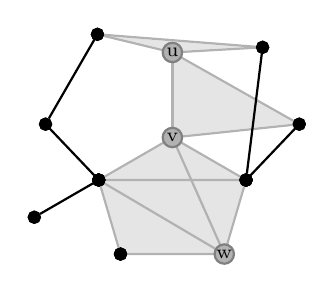
\begin{tikzpicture}[thick,scale=.54]
	\tikzstyle{pop}=[circle, draw, color=black!50,fill=black!30,text = black,
					inner sep=.0pt, minimum width=7pt]
	\tikzstyle{popi}=[circle, draw, color = black, fill=black,
					inner sep=0pt, minimum width=4pt]
	\tikzset{pil/.style={thick,color=black,shorten >=2.25pt}}
	\tikzset{pul/.style={thick,color=black!30,shorten >=2.25pt}}
	%%%Shadings
	\draw[fill=black!10,draw=white]
		(210+36:3)--(330-36:3)--(330:2)--(0:0)--(210:2)--cycle;
	\draw[fill=black!10,draw=white]
		(0:0)--(90:2)--(90+36:3)--(45:3)--(90:2)--(6:3)--cycle;
	%%% Grey Nodes and Edges
	\draw {(330-36:3) node[popi] {}edge[pul] (210:2) node[popi] {}};
	\draw {(210+36:3) node[popi] {} edge[pul] (330-36:3) node[popi] {}};
	\draw {(0:0) node[popi] {} edge[pul] (330-36:3) node[popi] {}};
	\draw {(330:2) node[popi] {} edge[pul] (330-36:3) node[popi] {}};
	\draw {(0:0) node[popi] {} edge[pul] (210:2) node[popi] {}};
	\draw {(210:2) node[popi] {} edge[pul] (330:2) node[popi] {}};
	\draw {(210:2) node[popi] {} edge[pul] (36+210:3) node[popi] {}};
	\draw {(0:0) node[popi] {} edge[pul] (330:2) node[popi] {}};
	\draw {(330-36:3) node[pop] {{\scriptsize{w}}}};
	%
	\draw {(0:0) node[popi] {} edge[pul] (90:2) node[popi] {}};
	\draw {(90:2) node[popi] {} edge[pul] (90+36:3) node[popi] {}};
	\draw {(90:2) node[popi] {} edge[pul] (6:3) node[popi] {}};
	\draw {(90+36:3) node[popi] {} edge[pul] (45:3) node[popi] {}};
	\draw {(45:3) node[popi] {} edge[pul] (90:2) node[popi] {}};
	\draw {(6:3) node[popi] {} edge[pul] (0:0) node[popi] {}};		
	\draw{(90:2) node[pop] {{\scriptsize{u}}}};
	\draw {(0:0) node[pop] {{\scriptsize{v}}}};
	%%% Black Nodes and Edges
	\draw {(210+36:3) node[popi] {}};
	\draw {(330:2) node[popi] {} edge[pil] (36+330:3) node[popi] {}};
	\draw {(210:2) node[popi] {} edge[pil] (210-36:3) node[popi] {}};
	\draw {(330:2) node[popi] {} edge[pil] (45:3) node[popi] {}};
	\draw {(210-36:3) node[popi] {} edge[pil] (90+36:3) node[popi] {}};
	\draw {(210:3.75) node[popi] {} edge[pil] (210:2) node[popi] {}};
\end{tikzpicture}
}
%%%%%%
%\tikzstyle{dendashed}=[dash pattern=on .3pt off .3pt]
\newcommand{\EqPathThreeRR}{%
\raisebox{-1pt}{
\tikz[scale=1,clip]{\draw[very thick,black!30,dir]
(180:.6) node[bnd]{{\scriptsize 1}}--
(    0, 0) node[bnd]{{\scriptsize 2}};
\draw[very thick,black!30,dir]
(    0, 0) node[bnd]{{\scriptsize 2}}--
(    0:.6) node[bnd]{{\scriptsize 3}};
}}\hspace{.75mm}
}
%%%%%%
\newcommand{\EqPathThreeRRR}{%
\raisebox{-2pt}{
\tikz[scale=.9,clip]{\draw[very thick,black!30,dir]
(180:.6) node[bnd]{{\scriptsize 1}}--
(    0, 0) node[bnd]{{\scriptsize 2}};
\draw[very thick,black!30,dir]
(    0, 0) node[bnd]{{\scriptsize 2}}--
(    0:.6) node[bnd]{{\scriptsize 3}};
}}\hspace{.75mm}
}
%%%%%%
\newcommand{\EqTriangleRRd}{%
\raisebox{-3mm}{
\tikz[scale=.5,clip]{\draw[very thick,black!30,dir]
(210:.6) node[bnd]{}--
(  90:.6) node[bnd]{{\scriptsize 2}};
\draw[very thick]
(  90:.6) node[bnd]{{\scriptsize 2}}--
( -30:.6) node[bnd]{{\scriptsize 3}};
\draw[very thick,black!30,dir]
( -30:.6) node[bnd]{{\scriptsize 3}}--
(210:.6) node[bnd]{{\scriptsize 1}};
}}\hspace{1.5mm}
}
%%%%%%
\newcommand{\EqTriangleRR}{%
\raisebox{-3mm}{
\tikz[scale=.5,clip]{\draw[very thick]
(210:.6) node[bnd]{}--
(  90:.6) node[brnd]{{\scriptsize 2}}--
( -30:.6) node[bnd]{{\scriptsize 3}}--
(210:.6) node[brnd]{{\scriptsize 1}};
}}\hspace{1.5mm}
}
%%%%%%
\newcommand{\EqPathFourRRd}{%
\raisebox{-1pt}{
\tikz[scale=.7,clip]{\draw[very thick,black!30,dir]
(180:  .6) node[bnd]{{\scriptsize 1}}--
(    0,   0) node[bnd]{{\scriptsize 2}};
\draw[very thick]
(    0,   0) node[bnd]{{\scriptsize 2}}--
(    0:  .6) node[bnd]{{\scriptsize 3}};
\draw[very thick,black!30,dir]
(    0:  .6) node[bnd]{{\scriptsize 3}}--
(    0:1.2) node[bnd]{{\scriptsize 4}};
}}\hspace{.75mm}
}
%%%%%%
\newcommand{\EqPathFourRR}{%
\raisebox{-2pt}{
\tikz[scale=.9,clip]{\draw[very thick,black!30,dir]
(180:  .6) node[bnd]{{\scriptsize 1}}--
(    0,   0) node[bnd]{{\scriptsize 2}};
\draw[very thick]
(    0,   0) node[bnd]{{\scriptsize 2}}--
(    0:  .6) node[bnd]{{\scriptsize 3}}--
(    0:1.2) node[bnd]{{\scriptsize 4}};
}}\hspace{.75mm}
}
%%%%%%
\newcommand{\EqSquareRRd}{%
\raisebox{-2.5mm}{
\tikz[scale=.45,clip]{\draw[very thick,black!30,dirs]
(225:.65) node[bnd]{}--
(135:.65) node[bnd]{{\scriptsize 2}};
\draw[very thick]
(135:.65) node[bnd]{{\scriptsize 2}}--
(  45:.65) node[bnd]{{\scriptsize 3}};
\draw[very thick,black!30,dirs]
(  45:.65) node[bnd]{{\scriptsize 3}}--
( -45:.65) node[bnd]{{\scriptsize 4}};
\draw[very thick]
( -45:.65) node[bnd]{{\scriptsize 4}}--
(225:.65) node[bnd]{{\scriptsize 1}};
}}\hspace{1.5mm}
}
%%%%%%
\newcommand{\EqSquareRR}{%
\raisebox{-3mm}{
\tikz[scale=.5,clip]{\draw[very thick,black!30,dirs]
(225:.65) node[bnd]{}--
(135:.65) node[bnd]{{\scriptsize 2}};
\draw[very thick]
(135:.65) node[bnd]{{\scriptsize 2}}--
(  45:.65) node[bnd]{{\scriptsize 3}}--
( -45:.65) node[bnd]{{\scriptsize 4}}--
(225:.65) node[bnd]{{\scriptsize 1}};
}}\hspace{1.5mm}
}
%%%%%%
\newcommand{\EqCompleteRR}{%
\raisebox{-3mm}{
\tikz[scale=.5,clip]{\draw[very thick,black!30,dirs]
(225:.65) node[bnd]{}--
(135:.65) node[bnd]{};
\draw[very thick,black!30,dirs]
(  45:.65) node[bnd]{}--
( -45:.65) node[bnd]{};
\draw[very thick]
(135:.65) node[bnd]{}--
( -45:.65) node[bnd]{};
\draw[very thick]
(  45:.65) node[bnd]{}--
(225:.65) node[bnd]{};
\draw[very thick]
(135:.65) node[bnd]{{\scriptsize 2}}--
(  45:.65) node[bnd]{{\scriptsize 3}};
\draw[very thick]
( -45:.65) node[bnd]{{\scriptsize 4}}--
(225:.65) node[bnd]{{\scriptsize 1}};
}}\hspace{1.5mm}
}
%%%%%%
\newcommand{\EqPathFourRRB}{%
\raisebox{-2pt}{
\tikz[scale=.9,clip]{\draw[very thick,black!30]
(    0:  .6) node[brnd]{{\scriptsize 3}}--
(    0:   0) node[brnd]{{\scriptsize 2}};
\draw[very thick]
(    0:   0) node[brnd]{{\scriptsize 2}}--
(180:  .6) node[bnd]{{\scriptsize 1}};
\draw[very thick]
(    0:  .6) node[brnd]{{\scriptsize 3}}--
(    0:1.2) node[bnd]{{\scriptsize 4}};
}}\hspace{.75mm}
}
%%%%%%
\newcommand{\EqCompleteSixRR}{%
\raisebox{-15pt}{
\tikz[scale=.8,clip]{
\foreach \x in {1,...,6}{
    \foreach \y in {1,...,6}{
    	\draw[very thick,black]
		(-60*\x+30:.6) -- (-60*\y+30:.6);}}
%%
\draw[ultra thick,black!30,dirs]
(150:.6) node[bnd]{{\scriptsize 1}}--
(210:.6) node[bnd]{{\scriptsize 2}};
%%
\draw[ultra thick,black!30,dirs]
( 30:.6) node[bnd]{{\scriptsize 5}}--
(-30:.6) node[bnd]{{\scriptsize 6}};
%%
\draw ( 90:.6) node[bnd]{{\scriptsize 3}};
\draw (-90:.6) node[bnd]{{\scriptsize 4}};
}}\hspace{1.75mm}
}
%%%%
%\item From the first item, with
%\[H_1^\dumbbell=(\{1,2,3,4\},\{12,23,24\},12)=\raisebox{-3.5mm}{
%\tikz[scale=.9,clip]{\draw[very thick,black!30]
%(180:.6) node[brnd]{{\scriptsize 1}}--
%(    0, 0) node[brnd]{{\scriptsize 2}};
%\draw[very thick]
%(    0, 0) node[brnd]{{\scriptsize 2}}--
%(  30:.6) node[bnd]{{\scriptsize 3}};
%\draw[very thick]
%(    0, 0) node[brnd]{{\scriptsize 2}}--
%( -30:.6) node[bnd]{{\scriptsize 4}};
%}}\hspace{1mm},\]
%then $\binom{(B{\bf 1})_e}{2}$ is the number of copies of $H_1^\dumbbell$ rooted at $e$.